\subsection{Interpreting Utilization}
\label{subsec:utilization}

The prime-time ratio showed that there is a possible change in behavior of the \test due to an increase in capacity from 105 Mbps to 250 Mbps. Now, we try to answer the question: \emph{Is there any change in user behavior due to the upgrade, and if so, where?}

\begin{figure}[ht!]
\centering
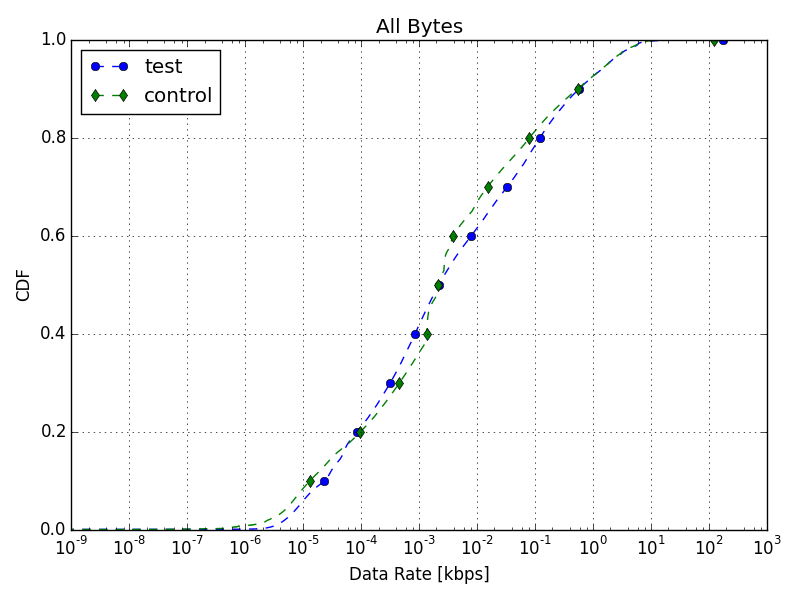
\includegraphics[width=0.90\linewidth]{figures/cdf-all-bytes.png}
  \caption{CDF of data rate per time slot for all devices (agg view of data): Overall not much change due to capacity increase. Median data rate ~ 2bps for 3 months x thousands of devices!}
  %http://sites.noise.gatech.edu/~sarthak/files/comcast/plots/full_dw/cdf-all-bytes.png
  \label{fig:CDF-data-rate-all}
\end{figure}

We compare the distribution of the data transferred per time slot for all devices in the \test and \control sets. Figure ~\ref{fig:CDF-data-rate-all} shows that the both sets have a very similar usage behavior distribution.

%%%%%%%%%%%%%%%%%%%%%%%%%%%%%%%%%%%%%%%%%%%%%%%%%%%%%%%%%%%%%%%%%%%%%
\begin{figure}[ht!]
%\hspace*{-0.2in}
\begin{minipage}{0.90\linewidth}
\centering
%
%\hfill
\begin{subfigure}[b]{0.90\linewidth}
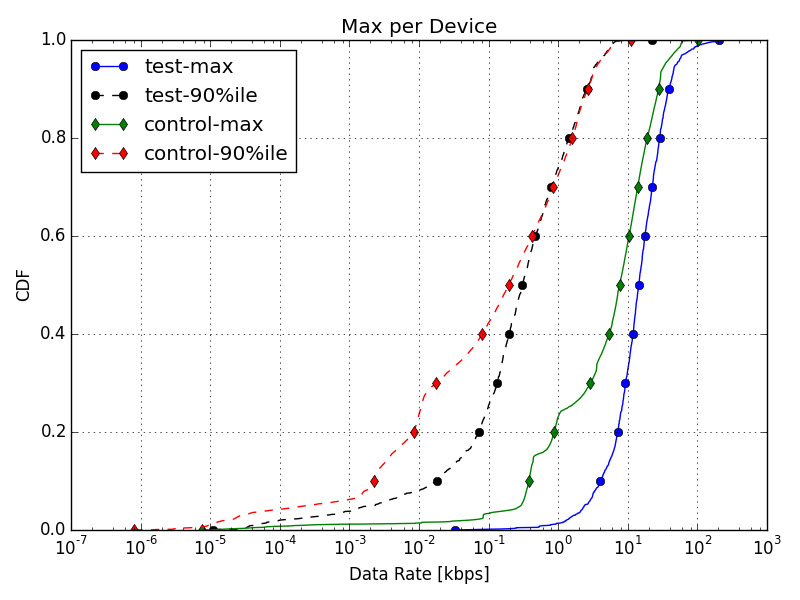
\includegraphics[width=\linewidth]{figures/cdf-max-per-device.png}
  \caption{CDF of max per device: test set has higher (max) average data rate below 10 kbps.  30\% of devices in the control set have a max data rate of 2 kbps while 30\% of test set has a max data rate of 10 kbps. (sanity check numbers, redo plot)}
  %http://sites.noise.gatech.edu/~sarthak/files/comcast/plots/full_dw/cdf-max-per-device.png
  \label{fig:CDF-data-rate-max}
\end{subfigure}
%
\vspace{-1em}
%
\begin{subfigure}[b]{0.90\linewidth}
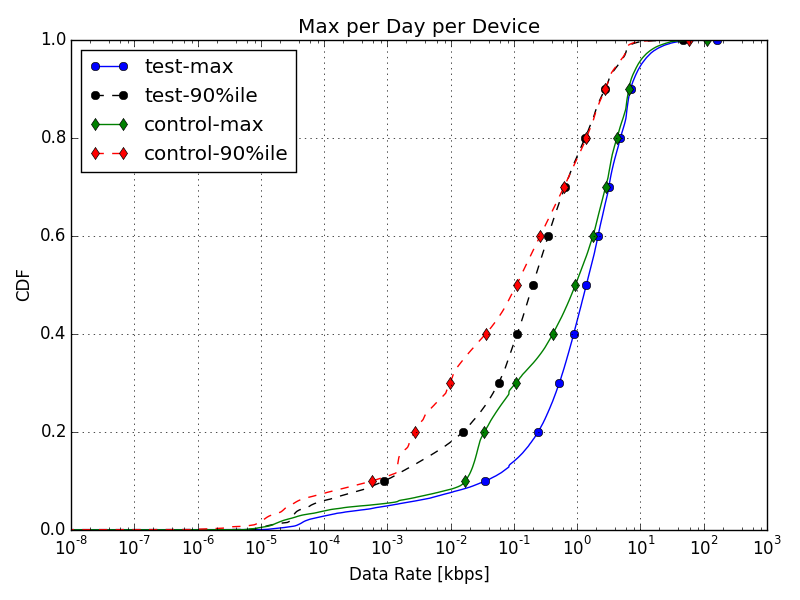
\includegraphics[width=\linewidth]{figures/cdf-max-per-day-per-device.png}
  \caption{CDF of max per device daily}
  \vspace{1em}
  %http://sites.noise.gatech.edu/~sarthak/files/comcast/plots/full_dw/cdf-max-per-day-per-device.png
  \label{fig:CDF-data-rate-max-daily}
\end{subfigure}
%\hfill
\end{minipage}
\caption{Peak Utilization: The maximum data rate varies for test and control set for low data rates, and this variation is present daily.}
\label{fig:peak-utilization}
% created using docs/metadata-separated.log
\end{figure}
%%%%%%%%%%%%%%%%%%%%%%%%%%%%%%%%%%%%%%%%%%%%%%%%%%%%%%%%%%%%%%%%%%%%%

Next we investigate the distribution of maximum data rate achieved by each household (figure~\ref{fig:CDF-data-rate-max}) over the three month period. Our results show that although the high utilizing households ($>$ 90\%-ile data rate) were similar throughout the set, showing no significant change in the maximum data rate, about 20\%-ile of the \test set devices saw a slight increase in the maximum data rate, which was much lower than link capacities. 
%the capacity utilization of both sets was similar during time slots with
% large data transfers, there is a certain difference in the maximum data
%rate per device for lower data rates \todo{needs a better more intuitive explanation}.

To confirm this behavior over each day, we plot the maximum data rate achieved \emph{daily} by each household (figure ~\ref{fig:CDF-data-rate-max-daily}). We observed that the maximum rate per device, for  devices with overall low usage , was higher for the \test set than the control set. We believe that this is an unbiased way to confirm the correlation between usage and capacity as the users were unaware of their increased capacity, nor did they require it. 
%The user's behavior does change when offered a higher capacity link,
%even though the overall capacity utilization stops increasing after a
%certain upper limit

We explore the reasons for such a consistent behavioral change: Discounting the possibility of this being a baseline behavior (i.e., \test set would show this even if it had the same capacity), we speculate that there could be two possible reasons for it: (1) short term downloads and/or web browsing achieves a slightly better data rate on a small time scale, or (2) real-time video quality is slightly higher, but not enough to completely saturate the access link capacity. Unfortunately, we miss these events due to a higher granularity of viewing data transferred only after 15 minutes.




\paragraph{Different Perspectives of Utilization: }We take this opportunity to reflect on the issue of increasing broadband availability, deployment, and adoption being faced by the FCC~\cite{fcc2015progress-report}. The network usage increases slightly for low link utilization, without the user actively changing his/her behavior to saturate the link capacity.

The user, and therefore the FCC (representing the users' rights and demands), and the ISPs, are both correct, but have a different perspective of broadband utilization and adoption; the slight change in behavior for low utilization could motivate a user to adopt a higher bandwidth tier. From the ISP perspective though, the users link capacity utilization does not show any change due to the upgrade in connectivity and is therefore a deterrent to offering the higher tier.

Vice versa, an ISP may tell the user that they need to upgrade their broadband access link to achieve higher data rate for low throughput periods too. And the user might not need it, as their link capacity is clearly not saturated. \todo{... doesn't make sense yet something missing ...}



\todo{this subsection needs a better transition to takeaway...}
% some conclusion
We recommend that the FCC add multiple benchmarks, including \sg{ ... what comes here?}
